\section{Model Selection}
Choosing the ML model that works the best for a given problem is a key factor for good results but it can be very time consuming. The following pages present the results obtained with several ML algorithms. Each method will be briefly introduced and tested using the training dataset. The results are analysed using three different tools:
\begin{itemize}
    \item Confusion matrix
    \item Precision, recall and F1 score
    \item ROC AUC Score
\end{itemize}
These three tools are presented and explained in Section \ref{model_tuning}.\\
Knowing the data is labeled all the methods but the last one are based on supervised learning.\\
Moreover it has already been demonstrated in Section \ref{balance_classes} that balancing classes dramatically improves results so the ML models are tested with an augmented training dataset containing duplicated individuals.

% \subsection{Stochastic Gradient Descent}

\subsection{Naive Bayes Classifier}
Naive Bayes classifiers use Bayes'theorem making the "naive" assumption that every pair of features are independant given the value of the class variable \cite{nbc_scikit} (i.e. \(P(x_i | y, x_1,..., x_{i-1}, x_{i+1},..., x_n) = P(x_i | y)\) ) leading to the following equality:
\[ P(y | x_1,..., x_n) = \frac{P(y)P(x_1,..., x_n | y)}{P(x_1,..., x_n)} = \frac{P(y)\prod_{i=1}^n P(x_i | y)}{P(x_1,..., x_n)} \]

The following results correspond to a Gaussian Naive Bayes\cite{nbcg_scikit} classifier that is very common when dealing with numerical continuous values. However it also assumes that every features follows a Gaussian distribution.\\

The confusion matrix in Figure \ref{nbd} shows poor results. This is expected because Figure \ref{data_analysis_1} demonstrates some features do not follow a Gaussian distribution. In addition, the assumption that features are independant from one another might not be relevant with this dataset. For instance, the \textit{snap\_ring\_peak\_force} might increase with the value of \textit{anlge\_1}.

\begin{figure}
    \center
    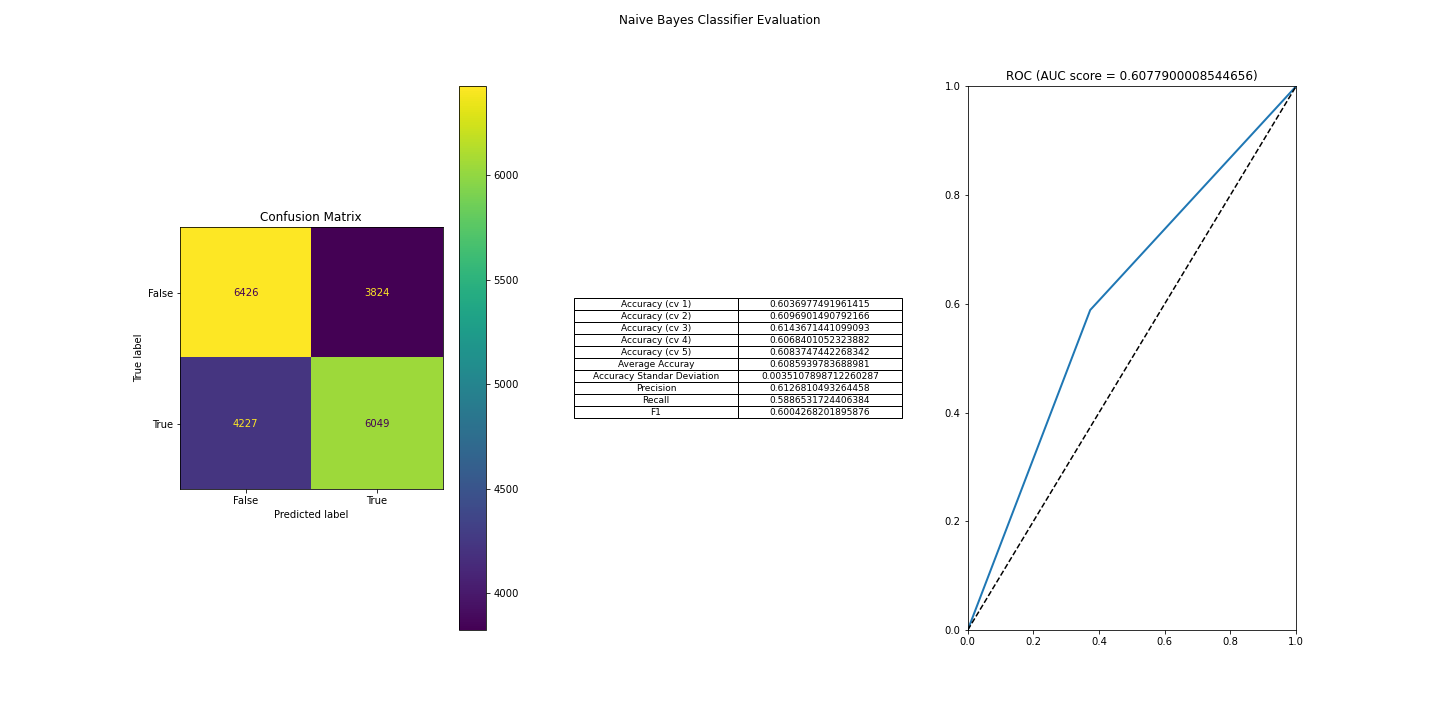
\includegraphics[scale=0.32]{img/nbc_d.png}
    \caption{Naive Bayes Classifier Evaluation}
    \label{nbc}
\end{figure}

\subsection{k-Nearest Neighbors}
The k-nearest neighbors algorithm works by classifiying an individual by looking at its neighbors \cite{knn_wikipedia}. The classifier simply look at the \(k\) nearest neighbors of the individual in the training population and attributes the class that correspond the best to the neighbors (the neighbors vote for their class, each vote is weighted either evenly accros the neighbors or according to the distance between the individual and the voting neighbor).\\

\begin{figure}
    \center
    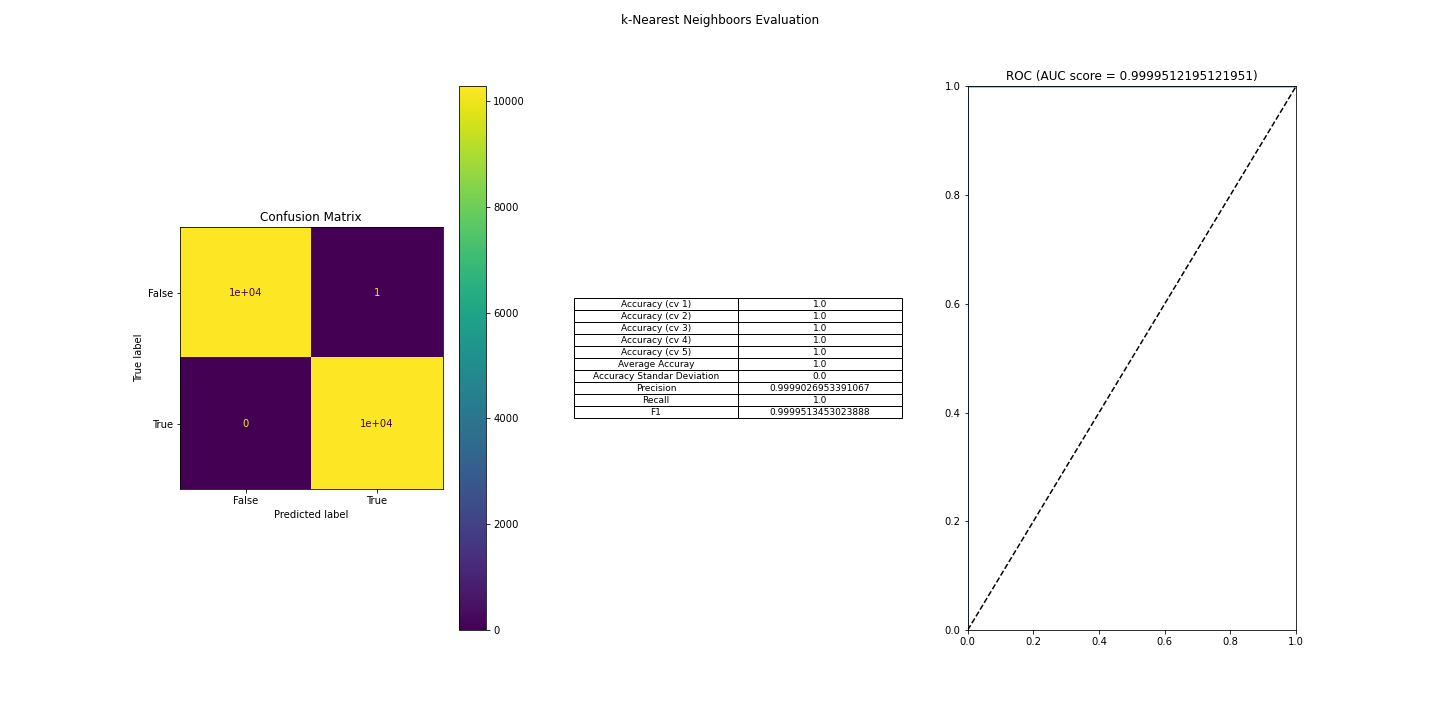
\includegraphics[scale=0.32]{img/knn_d.png}
    \caption{k-Nearest Neighbors Evaluation}
    \label{knn}
\end{figure}

\subsection{Random Forest Classifier}

\subsection{Multi-Layer Perceptron}

\subsection{Novelty Detection}